%# -*- coding: utf-8-unix -*-
%%==================================================
\chapter{产生式系统的搜索策略}\label{AIchap4}
%%%%%%%%%%%%%%%%%%%%%%%%%%%%%%%%%%%%
\begin{tcolorbox}[colback=white!50,colframe=orange!50,title=搜索]
    搜索是人工智能中的一个基本问题,并与推理密切相关, 搜索策略的优劣, 将直接影响到智能系统的性能与推理效率.\hfill
\end{tcolorbox}
%%%%-----------------------------------------
\begin{figure}[H]
    \centering
    \includegraphics[width=0.84\textwidth]{SS20191218004.jpg}
    \label{SS20191218004}
\end{figure}
%%%%%%%%%%%%%%%%%%%%%%%%%%%%%%%%%%
\section{搜索的基本概念}
    人工智能的任何问题的传统求解技术都离不开表示与搜索.
\subsection{搜索的含义}
%%%%%%%%%%%%%%%%%%%%%%%%%%%%%%%%%
\begin{mydef}{搜索}{1}
    依靠经验, 利用已有知识, 根据问题的实际情况, 不断寻找可利用知识, 从而构造一条代价最小的推理路线, 使问题得以解决的过程称为搜索.
\end{mydef}

\begin{itemize}
\item 适用情况: 不良结构或非结构化问题; 难以获得求解所需的全部信息; 更没有现成的算法可供求解使用.
\end{itemize}
%%%%-----------------------------------------
\section{搜索的类型}

    $\bullet$ 按是否使用启发式信息:
    \begin{itemize}
        \item 盲目搜索: 按预定的控制策略进行搜索, 在搜索过程中获得的中间信息并不改变控制策略.
        \item 启发式搜索: 在搜索中加入了与问题有关的启发性信息, 使得搜索朝着正确的方向进行, 加速问题的求解过程, 迅速找到最优解.
    \end{itemize}
    $\bullet$ 按问题的表示方式:
    \begin{itemize}
        \item 状态空间搜索是用状态空间法来求解问题而进行的搜索.
        \item 与或树搜索是用问题归约法来求解问题而进行的搜索.
    \end{itemize}
%%%%-----------------------------------------
\subsection{状态空间法}
\paragraph{状态空间表示方法}
\begin{itemize}
\item 状态(State): 是表示问题求解过程中每一步问题状况的数据结构, 它可表示为:
\begin{align}
    S_k=\{S_{k0}, S_{k1}, \cdots\},
\end{align}
当对每一个分量都给一确定的值时, 就得到了一个具体的状态.

\item 操作也称为\uwave{算符}, 它是把问题从一种状态变换为另一种状态的手段.
操作可以是一个机械步骤, 一个运算, 一条规则或一个过程. 操作可理解为状态集合上的一个函数, 它描述了状态之间的关系.

\item 状态空间: 描述一个问题的全部状态以及这些状态之间的相互关系. 常用三元组表示为:
\begin{align}
    (S, F, G),
\end{align}
其中, $S$为问题的所有初始状态集合; $F$为操作集合; $G$为目标状态集合.

\begin{remark}
    状态空间也可用一个赋值的有向图$G$来表示, 该有向图称为状态空间图. 在状态空间图中, 节点表示问题的状态, 有向边表示操作.
\end{remark}
\end{itemize}
%%%%-----------------------------------------
\paragraph{状态空间问题求解}
求解问题的基本过程:
\begin{itemize}
\item 首先为问题选择适当的“状态”及“操作”的形式化描述方法;
\item 然后从某个初始状态出发, 每次使用一个“操作”, 递增地建立起操作序列, 直到达到目标状态为止; 此时, 由初始状态到目标状态所使用的算符序列就是问题的一个解.
\end{itemize}
%%%%-----------------------------------------
\begin{example}
    \textbf{二阶梵塔问题}. 设有三根钢针, 它们的编号分别是1号、2号和3号. 在初始情况下, 1号钢针上穿有$A,B$两个金片, $A$比$B$小, $A$位于$B$的上面. 要求把这两个金片全部移到另一根钢针上, 而且规定每次只能移动一个金片, 任何时刻都不能使大的位于小的上面.
\end{example}
%%%%-----------------------------------------
\begin{result}
设用$S_k=(S_{k0}, S_{k1})$表示问题的状态, 其中, $S_{k0}$表示金片$A$所在的钢针号, $S_{k1}$表示金片$B$所在的钢针号.
全部可能的问题状态共有以下9种:
\begin{align}
\begin{array}{ll}
S_0&=(1, 1)\,\,   S_1=(1, 2)\,\,     S_2=(1, 3)\,\,    S_3=(2, 1)\,\,    S_4=(2, 2)\\
S_5&=(2, 3)\,\,   S_6=(3, 1) \,\,    S_7=(3, 2) \,\,   S_8=(3, 3).
\end{array}
\end{align}

\begin{itemize}
\item 问题的初始状态集合为$S=\{S_0\}$.
\item 目标状态集合为$G=\{S_4, S_8\}$.
\end{itemize}
%%%%%%%%%%%%%%%%%%%%%%%%%%%%%%%%%
初始状态$S_0$和目标状态$S_4$和$S_8$, 如图\ref{AI32fig2019120222}所示
%%%%-----------------------------------------
\begin{figure}[H]
    \centering
    \includegraphics[width=0.76\textwidth]{AI32C42019112501.PNG}
    \caption{二阶梵塔问题的初始状态和目标状态}
    \label{AI32fig2019120222}
\end{figure}
%%%%-----------------------------------------
操作分别用$A(i, j)$和$B(i, j)$表示, 意义如下:
\begin{itemize}
\item  $A(i, j)$表示把金片$A$从第$i$号钢针移到$j$号钢针上;
\item  $B(i, j)$表示把金片$B$从第$i$号钢针移到第$j$号钢针上. 共有12种操作, 它们分别是:
\begin{align}
\begin{array}{ll}
      A(1, 2)\,\,   A(1, 3) \,\,    A(2, 1)\,\,     A(2, 3) \,\,    A(3, 1) \,\,    A(3, 2),\\
      B(1, 2)\,\,     B(1, 3) \,\,     B(2, 1)\,\,     B(2, 3)  \,\,   B(3, 1)  \,\,    B(3, 2).
\end{array}
\end{align}
\end{itemize}
根据上述9种可能的状态和12种操作, 可构成二阶梵塔问题的状态空间图, 如图 \ref{AI32fig2019120223} 所示.
从初始节点(1, 1)到目标节点(2, 2)及(3, 3)的任何一条路径都是问题的一个解. 其中, 最短的路径长度是3, 它由3个操作组成.
\end{result}

%%%%-----------------------------------------
\begin{example}
从 (1,1)开始, 通过使用操作$A(1, 3),B(1, 2)$及$A(3, 2)$, 可到达 (3, 3).
%%%%-----------------------------------------
\begin{figure}[H]
\centering
\includegraphics[width=0.6\textwidth]{AI32C42019112502.PNG}
\caption{二阶梵塔的状态空间图}
\label{AI32fig2019120223}
\end{figure}
\end{example}
%%%%-----------------------------------------
\begin{think}
    用matlab或Python语言实现图 \ref{AI32fig2019120223}的二阶梵塔问题的程序, 并绘制流程图.
\end{think}
%%%%-----------------------------------------
\begin{example}
  修道士(Missionaries)和野人(Cannibals)问题(简称M-C问题). 设在河的一岸有三个野人、三个修道士和一条船, 修道士想用这条船把所有的人运到河对岸, 但受以下条件约束:
\begin{itemize}
\item 修道士和野人都会划船, 但每次船上至多可载两个人;
\item 在河的任一岸, 如果野人数目超过修道士数, 修道士会被野人吃掉.
\end{itemize}

如果野人会服从任何一次过河安排, 请规划一个确保修道士和野人都能过河, 且没有修道士被野人吃掉的安全过河计划.
\end{example}
%%%%%%%%%%%%%%%%%%%%%%%%%%%%%%%%%%
\begin{result}
首先选取描述问题状态的方法. 在这个问题中, 需要考虑两岸的修道士人数和野人数, 还需要考虑船在左岸还是在右岸. 从而可用一个三元组来表示相应的状态
         $$S=(m, c, b),$$
其中, $m$表示左岸的修道士人数, $c$表示左岸的野人数, $b$表示左岸的船数.
右岸的状态可由下式确定:
\begin{itemize}
\item 右岸修道士数  $m'=3-m$.
\item 右岸野人数   $ c'=3-c$.
\item 右岸船数      $b'=1-b$.
\end{itemize}
在这种表示方式下, $m\in \{0,1,2,3\}$和$c\in \{0,1,2,3\}$, $b\in \{0,1\}$可取其中之一. 因此, 三元组共有$4\times 4\times 2=32$种状态.

这32种状态并非全有意义, 除去不合法状态和修道士被野人吃掉的状态, 有意义的状态只有16种:
\begin{align*}
        &S_0=(3, 3, 1)  &S_1=(3, 2, 1)     &\,\,S_2=(3, 1, 1)&S_3=(2, 2, 1)\\
        &S_4=(1, 1, 1)  &S_5=(0, 3, 1)     &\,\,S_6=(0, 2, 1)&S_7=(0, 1, 1)\\
        &S_8=(3, 2, 0)  &S_9=(3, 1, 0)     &\,\,S_{10}=(3, 0, 0)&S_{11}=(2, 2, 0)\\
        &S_{12}=(1, 1,0)&\,\,\,S_{13}=(0, 2, 0)  &\,\,S_{14}=(0, 1, 0)&\,\,\,S_{15}=(0, 0, 0).
\end{align*}
有了这些状态, 还需要考虑可进行的操作.

%%%%%%%%%%%%%%%%%%%%%%%%%%%%%%%%%
\begin{mydef}{操作}{1}
    是指用船把修道士或野人从河的左岸运到右岸, 或从河的右岸运到左岸.
\end{mydef}

每个操作都应当满足如下条件:
\begin{itemize}
\item 一是船至少有一个人($m$或$c$)在操作, 离开岸边的$m$和$c$的减少数目应该等于到达岸边的$m$和$c$的增加数目;
\item 二是每次操作下的船上人数不得超过2个;
\item 三是操作应保证不产生非法状态.
\end{itemize}
因此, 操作应由条件部分和动作部分:
\begin{itemize}
\item 动作刻划了应用此操作所产生的结果,
\item 条件只有当其条件具备时才能使用.
\end{itemize}
\begin{remark}
    符号$P_{ij}$表示从左岸到右岸的运人操作, 符号$Q_{ij}$表示从右岸到左岸的操作, 其中$i$表示船上的修道士人数, $j$表示船上的野人数.
本问题的操作集由10种操作组成:
\begin{align}
  F=\{P_{01}, P_{10}, P_{11}, P_{02}, P_{20},Q_{01}, Q_{10}, Q_{11}, Q_{02}, Q_{20}\}.
\end{align}
\end{remark}

下面以$P_{01}$和$Q_{01}$为例来说明这些操作的条件和动作, 如表\ref{Tabexam4.1}.
\begin{table}
\begin{center}
\caption{操作的条件和动作表}
\label{Tabexam4.1}
\begin{tabular}{lcccc}
\hline
  % after \\: \hline or \cline{col1-col2} \cline{col3-col4} ...
操作符号                  &  条件                                                                              &  动作\\
\hline
$P_{01}$     &  $b=1, m=0$或$3, c\geq 1$        &  $b=0, c=c-1$\\
$Q_{01}$     &  $b=0, m=0$或$3, c\leq 2 $         &  $b=1, c=c+1$\\
\hline
\end{tabular}
\end{center}
\end{table}
\end{result}
%%%%-----------------------------------------
\begin{example}
    猴子摘香蕉问题. 在讨论谓词逻辑知识表示时, 我们曾提到过这一问题, 现在用状态空间法来解决这一问题.
\end{example}
\begin{result}
问题的状态可用4元组$(w, x, y, z)$表示, 其中:
\begin{itemize}
    \item $w$表示猴子的水平位置;
    \item $x$表示箱子的水平位置;
    \item $y$表示猴子是否在箱子上, 当猴子在箱子上时, $y=1$, 否则$y=0$;
    \item $z$表示猴子是否拿到香蕉, 当拿到香蕉时$z=1$, 否则$z=0$.
\end{itemize}
所有可能的状态为
\begin{itemize}
    \item $S_0: (a, b, 0, 0)$;    初始状态;
    \item $S_1: (b, b, 0, 0)$;
    \item $S_2: (c, c, 0, 0)$;
    \item $S_3: (c, c, 1, 0)$;
    \item $S_4: (c, c, 1, 1)$;    目标状态.
\end{itemize}
允许的操作为
\begin{itemize}
    \item Goto($u$): 猴子走到位置$u$, 即$(w, x, 0, 0) \rightarrow (u, x, 0, 0)$.
    \item Pushbox($v$): 猴子推着箱子到水平位置$v$, 即$(x, x, 0, 0) \rightarrow (v, v, 0, 0)$.
    \item Climbbox: 猴子爬上箱子, 即$(x, x, 0, 0) \rightarrow (x, x, 1, 0)$.
    \item Grasp: 猴子拿到香蕉, 即$(c, c, 1, 0 ) \rightarrow (c, c, 1, 1)$.
\end{itemize}
这个问题的状态空间图如图\ref{AI32fig2019120224}所示. 不难看出, 由初始状态变为目标状态的操作序列为:
\begin{center}
  \{Goto($b$), Pushbox($c$), Climbbox, Grasp\}.
\end{center}
%%%%-----------------------------------------
\begin{figure}[H]
\centering
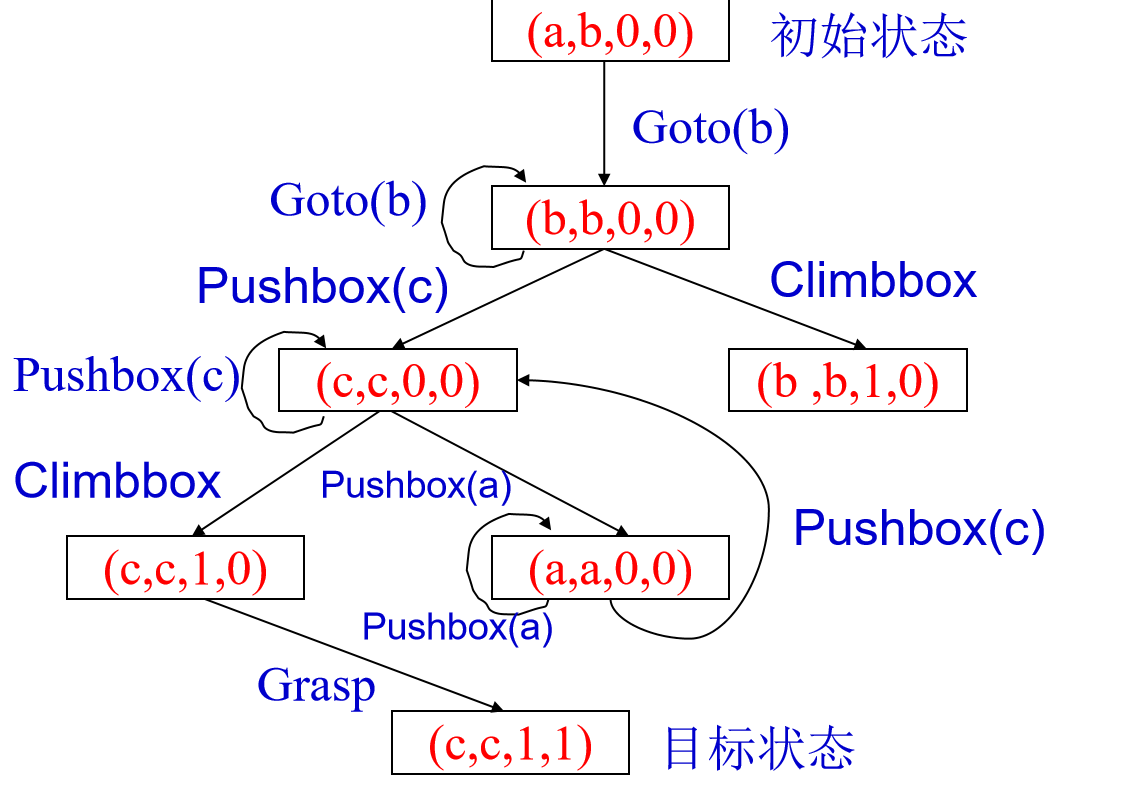
\includegraphics[width=0.6\textwidth]{AI32C42019112503.PNG}
\caption{猴子摘香蕉问题的状态空间图}
\label{AI32fig2019120224}
\end{figure}
%%%%-----------------------------------------
解序列为: \{Goto(b), Pushbox(c), Climbbox, Grasp\}.
\end{result}
%%%%%%%%%%%%%%%%%%%%%%%%%%%%%%%%%%
\subsection{问题归约法}
%%%%%%%%%%%%%%%%%%%%%%%%%%%%%%%%%%
\subsubsection{问题的分解与等价变换}
当一个问题比较复杂时, 可通过分解或变换, 将其转化为一系列较简单的子问题, 然后通过对这些子问题的求解, 来实现对原问题的求解.
\subparagraph{问题的分解}
如果一个问题$P$可以归约为一组子问题$P_1,P_2,\cdots,P_n$, 并且只有当所有子问题$P_i$都有解时, 原问题$P$才有解; 任何一个子问题$P_i$无解, 都会导致原问题$P$无解, 则称此种归约为问题的分解.
即分解所得到的子问题的“与”与原问题$P$等价.
%%%%%%%%%%%%%%%%%%%%%%%%%%%%%%%%%%
\subparagraph{等价变换}
如果一个问题$P$可以归约为一组子问题$P_1,P_2,\cdots,P_n$, 并且子问题$P_i$中只要有一个有解, 则原问题$P$就有解, 只有当所有子问题$P_i$都无解时原问题$P$才无解, 称此种归约为问题的等价变换, 简称变换.
即变换所得到的子问题应与原问题$P$等价.

(1) \textbf{与树分解}
%%%%-----------------------------------------
\begin{figure}[H]
\centering
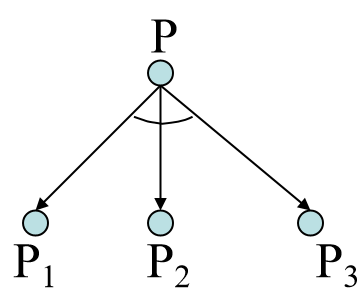
\includegraphics[width=0.2\textwidth]{yushu2019112525.PNG}
\caption{与树 }
\label{AI32fig25}
\end{figure}
%%%%-----------------------------------------

(2) \textbf{或树——等价变换}
%%%%-----------------------------------------
\begin{figure}[H]
    \centering
    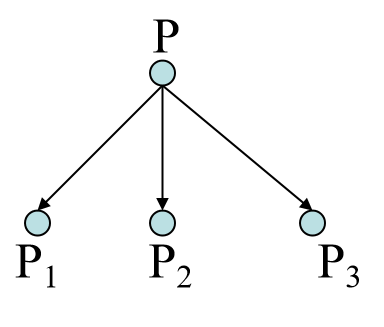
\includegraphics[width=0.2\textwidth]{yushu2019112526.PNG}
    \caption{或树 }
    \label{AI32fig26}
\end{figure}
%%%%-----------------------------------------

(3) \textbf{与/或树}
%%%%-----------------------------------------
\begin{figure}[H]
    \centering
    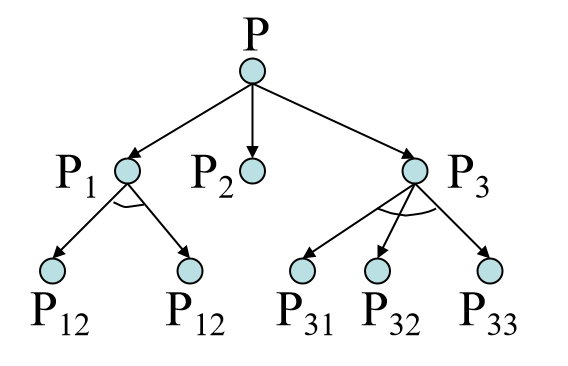
\includegraphics[width=0.25\textwidth]{yushu2019112527.PNG}
    \caption{与/或树 }
    \label{AI32fig27}
\end{figure}
%%%%-----------------------------------------
(4) \textbf{端节点与终止节点}\,\, 在与/或树中, 没有子节点的节点称为端节点; 本原问题所对应的节点称为终止节点. 可见, 终止节点一定是端节点, 但端节点却不一定是终止节点.

(5) \textbf{可解节点与不可解节点}
\begin{mydef}{可解节点}{1}
在与/或树中, 可解节点是满足以下三个条件之一的节点:

\ding{172} 任何终止节点都是可解节点.

\ding{173} 对“或”节点, 当其子节点中至少有一个为可解节点时, 则该或节点就是可解节点.

\ding{174} 对“与”节点, 只有当其子节点全部为可解节点时, 该与节点才是可解节点.
\end{mydef}

\begin{mydef}{不可解节点}{1}
\ding{172} 不为终止节点的端节点是不可解节点.

\ding{173} 对“或”节点, 若其全部子节点都为不可解节点, 则该或节点是不可解节点.

\ding{174} 对“与”节点, 只要其子节点中有一个为不可解节点, 则该与节点是不可解节点.
\end{mydef}

(6) \textbf{解树} 由可解节点构成, 由这些可解节点可以推理出初始节点, 可解节点的子树为解树. 在解树中一定包含初始节点.
%%%%---------------------------------------------
\begin{example}
    图 \ref{AI32fig28} 给出的与或树中, 用红 线表示的子树是一个解树. 在图 \ref{AI32fig28} 中, 节点$P$为原始问题节点, 用$t$标出的节点是终止节点. 根据可解节点的定义, 很容易推出原始问题$P$为可解节点.
\end{example}
%%%%---------------------------------------------
\begin{remark}
    问题归约的求解过程实际上就是生成解树, 即证明原始节点是可解节点的过程. 这一过程涉及到搜索的问题, 对于与/或树的搜索将在后面详细讨论.
\end{remark}
%%%%-----------------------------------------
\begin{figure}[H]
    \centering
    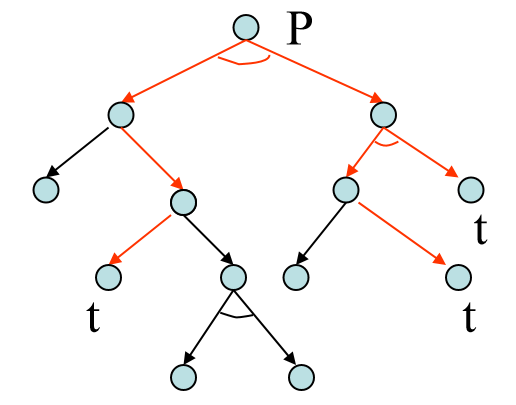
\includegraphics[width=0.3\textwidth]{yushu2019112528.PNG}
    \caption{与/或树 }
    \label{AI32fig28}
\end{figure}
%%%%-----------------------------------------
\begin{example}
    \Circled{\textbf{三阶梵塔问题}} 要求把1号钢针上的3个金片全部移到3号钢针上, 如图\ref{AI32fig29}所示.
\end{example}
\begin{answer}
本例用归约法来解决问题.
为了能够解决这一问题, 首先需要定义该问题的形式化表示方法.
设用三元组$(i, j, k)$表示问题在任一时刻的状态, 用“$\rightarrow$”表示状态的转换. 上述三元组$(i, j, k)$的意思分别为:
\begin{itemize}
    \item $i$ 代表金片$C$所在的钢针号;
    \item $j$ 代表金片$B$所在的钢针号;
    \item $k$ 代表金片$A$所在的钢针号.
\end{itemize}
%%%%-----------------------------------------
\begin{figure}[H]
    \centering
    \includegraphics[width=0.8\textwidth]{yushu2019112529.PNG}
    \caption{三阶汉诺塔问题 }
    \label{AI32fig29}
\end{figure}
%%%%-----------------------------------------
利用问题归约方法, 原问题可分解为以下三个子问题:

(1) 把金片$A$及$B$移到2号钢针上的双金片移动问题. 即(1, 1, 1)$\rightarrow$(1, 2, 2);

(2) 把金片$C$移到3号钢针上的单金片移动问题. 即 (1, 2, 2)$\rightarrow$(3, 2, 2);

(3) 把金片$A$及$B$移到3号钢针的双金片移动问题. 即(3, 2, 2)$\rightarrow$(3, 3, 3), 其中, 子问题(1)和(3)都是一个二阶梵塔问题, 它们都还可以再继续进行分解; 子问题(2)是本原问题, 它已不需要再分解.

三阶梵塔问题的分解过程可用图 \ref{AI32fig2019120230} 的与/或树表示.
在该与/或树中, 有7个终止节点, 它们分别对应着7个本原问题. 如果把这些本原问题从左至右排列起来, 即得到了原始问题的解:
\begin{center}
(1, 1, 1)$\rightarrow$(1, 3, 3),\,(1, 3, 3)$\rightarrow$(1, 2, 3),\,(1, 2, 3)$\rightarrow$(1, 2, 2),\,(1, 2, 2)$\rightarrow$(3, 2, 2),

(3, 2, 2)$\rightarrow$(3, 2, 1),\,(3, 2, 1)$\rightarrow$(3, 3, 1),\,(3, 3, 1)$\rightarrow$(3, 3, 3).
\end{center}
%%%%-----------------------------------------
\begin{figure}[H]
    \centering
    \includegraphics[width=0.76\textwidth]{yushu2019112530.PNG}
    \caption{与/或树 }
    \label{AI32fig2019120230}
\end{figure}
\end{answer}
%%%%-----------------------------------------
\section{状态空间的盲目搜索}
%%%%-----------------------------------------
\subsection{一般图搜索过程}
1) 先把问题的初始状态作为当前扩展节点, 对其进行扩展, 生成一组子节点;

2) 检查问题的目标状态是否出现在这些子节点中.

\qquad\ding{172} 若出现, 则搜索成功, 找到了问题的解;

\qquad\ding{173} 否则, 按照某种搜索策略从已生成的子节点中选择一个节点作为当前扩展节点.

3) 重复上述过程, 直到目标状态出现在子节点中或者没有可供操作的节点为止.

\begin{remark}
    所谓对一个节点进行“扩展”是指对该节点用某个可用操作进行作用, 生成该节点的一组子节点.
\end{remark}

算法的数据结构和符号约定
%%%%-----------------------------------------
\begin{itemize}
\item Open表: 用于存放刚生成的节点;
\item Closed表: 用于存放已经扩展或将要扩展的节点;
\item $S_0$: 表示问题的初始状态;
\item $G$: 表示搜索过程所得到的搜索图;
\item $M$: 表示当前扩展节点新生成的且不为自己先辈的子节点集.
\end{itemize}

\textbf{一般图搜索过程}

\quad (1) 把初始节点$S_0$放入Open表, 并建立目前仅包含$S_0$的图$G$;

\quad (2) 检查Open表是否为空, 若为空, 则问题无解, 失败退出;

\quad (3) 把Open表的第一个节点取出放入Closed表, 并记该节点为$n$;

\quad (4) 考察节点$n$是否为目标节点. 若是, 则得到了问题的解, 成功退出;

\quad (5) 扩展节点$n$, 生成一组子节点. 把这些节点中不是节点$n$先辈的那部分子节点加入集合$M$, 并把这些子节点作为节点$n$的子节点加入$G$中.

\quad (6) 针对$M$中子节点的不同情况, 分别作如下处理:

    \quad \quad \ding{172} 对那些没有在$G$中出现过的$M$成员, 设置一个指向其父节点(即节点$n$)的指针, 并把它放入Open表. (新生成的).

    \quad \quad \ding{173} 对那些原来已在$G$中出现过, 但还没有被扩展的$M$成员, 确定是否需要修改它指向父节点的指针. (原来生成但未扩展的).

    \quad \quad \ding{174} 对于那些先前已在$G$中出现过, 并已经扩展了的$M$成员, 确定是否需要修改其后继节点指向父节点的指针. (原来生成也扩展过的).

\quad (7) 按某种策略对Open表中的节点进行排序.

\quad (8) 转第(2)步.
%%%%------------------------------------------------
\begin{remark}
    上述过程是状态空间的一般图搜索算法, 它具有通用性, 后面所要讨论的各种状态空间搜索策略都是上述过程的一个特例. 各种搜索策略的主要区别在于\uwave{对Open表中节点的排列顺序的方式不同}.
\end{remark}

%%%%------------------------------------------------
\begin{remark}

(1) 广度优先搜索把先生成的子节点排在前面, 而深度优先搜索则把后生成的子节点排在前面.

(2) 在第(5)步对节点$n$扩展后, 生成并记入$M$的子节点有以下三种情况:

    \quad \ding{172} 该子节点来从未被任何节点生成过, 由$n$第一次生成;

    \quad \ding{173} 该子节点原来被其他节点生成过, 但还没有被扩展, 这一次又被$n$再次生成;

    \quad \ding{174} 该子节点原来被其他节点生成过, 并且已经被扩展过, 这一次又被$n$再次生成.

以上三种情况是对一般图搜索算法而言的.

对于盲目搜索, 由于其状态空间是树状结构, 因此不会出现后两种情况, 每个节点经扩展后生成的子节点都是第一次出现的节点.

\begin{tcolorbox}
    盲目搜索不必检查并修改指向父节点的指针.
\end{tcolorbox}

(3) 在第(6)步针对$M$中子节点的不同情况进行处理时, 如果发生当第②种情况, 那么, 这个$M$中的节点究竟应该作为哪一个节点的后继节点呢?
一般是由原始节点到该节点路径上所付出的代价来决定的, 哪一条路经付出的代价小, 相应的节点就作为它的父节点. 所谓由原始节点到该节点路径上的代价是指这条路经上的所有有向边的代价之和.

如果发生第\ding{174}种情况, 除了需要确定该子节点指向父节点的指针外, 还需要确定其后继节点指向父节点的指针. 其依据也是由原始节点到该节点的路径上的代价.

(4) 在搜索图中, 除初始节点外, 任意一个节点都含有且只含有一个指向其父节点的指针. 因此, \uwave{由所有节点及其指向父节点的指针所构成的集合是一棵树, 称为搜索树}.

(5) 在搜索过程的第(4)步, 一旦某个被考察的节点是目标节点, 则搜索过程成功结束. 由初始节点到目标节点路径上的所有操作就构成了该问题的解, 而路径由第(6)步所形成的指向父节点的指针来确定.

(6) 如果搜索过程终止在第(2)步, 即没有达到目标, 且\textup{Open}表中已无可供扩展的节点, 则失败结束.
\end{remark}
%%%%-----------------------------------------
\subsection{广度优先和深度优先搜索}
%%%%---------------------------------
\subsubsection{广度优先搜索}
\subparagraph{基本思想}
    从初始节点$S_0$开始逐层向下扩展, 在第$n$层节点还没有全部搜索完之前, 不进入第$n+1$层节点的搜索方式. Open表中的节点总是按进入的先后排序, 先进入的节点排在前面, 后进入的节点排在后面.
%%%%-----------------------------------------
\subparagraph{搜索算法} 具体流程如下:

\quad (1) 把初始节点$S_0$放入Open表中;

\quad (2) 如果Open表为空, 则问题无解, 失败退出;

\quad (3) 把Open表的第一个节点取出, 放入Closed表, 并记该节点为$n$;

\quad (4) 考察节点$n$是否为目标节点. 若是, 则得到问题的解, 成功退出;

\quad (5) 若节点$n$不可扩展, 则转第(2)步;

\quad (6) 扩展节点$n$, 将其子节点放入Open表的尾部, 并为每一个子节点设置指向父节点的指针, 然后转第(2)步.
%%%%-----------------------------------------
\begin{example}
\textbf{$3\times 3$的方格棋盘上的八数码难题}\quad 如图\ref{AI32fig2019120231}所示, 表上放置了标有数字1、2、3、4、5、6、7、8的八张牌, 初始状态$S_0$, 目标状态$S_g$. 可以使用的操作有
\begin{center}
    空格左移, 空格上移, 空格右移, 空格下移,
\end{center}
即只允许把位于空格左、上、右和下方的牌移入空格. 要求应用广度优先搜索策略寻找从初始状态到目标状态的解路径.
\end{example}
%%%%-----------------------------------------
\begin{figure}[H]
    \vspace{-0.5cm}
    \centering
    \includegraphics[width=0.45\textwidth]{yushu2019112531.PNG}
    \caption{与/或树 }
    \label{AI32fig2019120231}
\end{figure}
%%%%-----------------------------------------
\begin{figure}[H]
    \centering
    \includegraphics[width=0.7\textwidth]{yushu2019112532.PNG}
    \caption{与/或树 }
    \label{AI32fig32}
\end{figure}
%%%%-----------------------------------------
\subsubsection{深度优先搜索}
%%%%-----------------------------------------
\subparagraph{基本思想}
    从初始节点$S_0$开始, 在其子节点中选择一个最新生成的节点进行考察, 如果该子节点不是目标节点且可以扩展, 则扩展该子节点, 然后再在此子节点的子节点中选择一个最新生成的节点进行考察;
    依此向下搜索, 直到某个子节点既不是目标节点, 又不能继续扩展时, 才选择其兄弟节点进行考察.
%%%%-----------------------------------------
\subparagraph{算法描述}~{}

\quad   (1) 把初始节点$S_0$放入Open表中;

\quad   (2) 如果Open表为空, 则问题无解 , 失败退出;

\quad   (3) 把Open表的第一个节点取出, 放入Closed表, 并记该节点为$n$;

\quad   (4) 考察节点$n$是否为目标节点. 若是, 则得到问题的解, 成功退出;

\quad   (5) 若节点$n$不可扩展, 则转第(2)步;

\quad   (6) 扩展节点$n$, 将其子节点放入Open表的首部, 并为每一个子节点设置 指向父节点的指针, 然后转第(2)步.
%%%%-----------------------------------------%
\begin{example}
    \Circled{八数码难题}\quad 八数码难题的深度优先搜索如右图\ref{AI32fig33}.
\end{example}
%%%%-----------------------------------------
\begin{figure}[H]
    \centering
    \includegraphics[angle=90,width=0.6\textwidth]{yushu2019112533.PNG}
    \caption{深度优先搜索(不完全图) }
    \label{AI32fig33}
\end{figure}
%%%%-----------------------------------------
\begin{remark}
    有界深度优先搜索算法是一种改进的深度优先算法, 将其深度限制为$d_m$.
\end{remark}
%%%%-----------------------------------------
\subsection{代价树搜索}
%%%%-----------------------------------------
\subsubsection{代价树的广度优先搜索}
    在代价树中, 可以用$g(n)$表示从初始节点$S_0$到节点$n$的代价, 用$c(n_1, n_2)$表示从父节点$n_1$到其子节点$n_2$的代价.
这样, 对节点$n_2$的代价有: $g(n_2)=g(n_1)+c(n_1, n_2)$. 代价树搜索的目的是为了找到最佳解(即找一条代价最小的解路径).
%%%%-----------------------------------------
\subsubsection{代价树的广度优先搜索算法}

\textbf{广度优先搜索算法的流程描述}:

\quad (1) 把初始节点$S_0$放入Open表中, 置$S_0$的代价$g(S_0)=0$;

\quad (2) 如果Open表为空, 则问题无解 , 失败退出;

\quad (3) 把Open表的第一个节点取出, 放入Closed表, 并记该节点为$n$;

\quad (4) 考察节点$n$是否为目标. 若是, 则找到了问题的解, 成功退出;

\quad (5) 若节点$n$不可扩展, 则转第(2)步;

\quad (6) 扩展节点$n$, 生成其子节点$n_i\,(i=1, 2, \cdots)$, 将这些子节点放入Open表中, 并为每一个子节点设置指向父节点的指针. 按如下公式:
\begin{align}
    g(n_i)=g(n)+c(n_i),\,\,i=1,2,...
\end{align}
计算各子结点的代价, 并根据各子结点的代价对Open表中的全部结点按代价由小到大的顺序排序. 然后转第(2)步.
%%%%%%%%%%%%%%%%%%%%%%%%%%%%%%%%%%%%%%%
\begin{example}
    (\textbf{城市交通问题}) 设有5个城市, 它们之间的交通线路如左侧子图\ref{AI32fig2019120234}所示, 图中的数字表示两个城市之间的交通费用, 即代价. 用代价树的广度优先搜索, 求从$A$市出发到$E$市, 费用最小的交通路线.
\end{example}
%%%%%%%%%%%%%%%%%%%%%%%%%%%%%%%%%%
\begin{result}
%%%%-----------------------------------------
\begin{figure}[H]
    \centering
    \includegraphics[width=0.38\textwidth]{yushu2019112534.PNG}
    \includegraphics[width=0.35\textwidth]{yushu2019112535.PNG}
    \caption{城市交通图(左子图), 城市交通图的广度优先代价树 (右子图)}
    \label{AI32fig2019120234}
\end{figure}
代价树如右侧子图\ref{AI32fig2019120234}所示. 红线为最优解, 其代价为8.
%%%%-----------------------------------------
\subsubsection{代价树的深度优先搜索算法}~{}

\quad (1) 把初始节点$S_0$放入Open表中, 置$S_0$的代价$g(S_0)=0$;

\quad (2) 如果Open表为空, 则问题无解 , 搜索算法失败, 退出;

\quad (3) 把Open表的第一个节点取出放入Closed表, 并记该节点为$n$;

\quad (4) 考察节点$n$是否为目标节点. 若是, 则找到了问题的解, 搜索算法成功退出;

\quad (5) 若节点$n$不可扩展, 则转第(2)步;

\quad (6) 扩展节点$n$, 生成其子节点$n_i,\,(i=1, 2,\cdots)$, 将这些子节点按边代价由小到大放入Open表的首部, 并为每一个子节点设置指向父节点的指针. 然后转第(2)步.
\end{result}
%%%%-----------------------------------------
\section{搜索策略}
%%%%-----------------------------------------
\subsection{状态空间的启发式搜索}
%%%%-----------------------------------------
\begin{mydef}{启发性信息}{1}
    启发性信息是指那种与具体问题求解过程有关, 并可指导搜索过程朝着最有希望方向前进的控制信息.
\end{mydef}

%%%%-----------------------------------------
\paragraph{启发性信息的种类}
\begin{itemize}
\item 有效地确定扩展节点的信息;
\item 有效地决定哪些后继节点应被生成的信息;
\item 能决定在扩展一个节点时哪些节点应从搜索树上删除的信息.
\end{itemize}
%%%%-----------------------------------------
\paragraph{启发性信息的作用} 启发信息的启发能力越强, 扩展的无用结点越少.

\begin{mydef}{估价函数}{1}
    估价函数是用来估计节点重要性的函数.
\end{mydef}
估价函数$f(n)$被定义为从初始节点$S_0$出发, 约束经过节点$n$到达目标节点$S_g$的所有路径中最小路径代价的估计值. 它的一般形式为:
\begin{align}
    f(n)=g(n)+h(n),
\end{align}
其中, $g(n)$是从初始节点$S_0$到节点$n$的实际代价; $h(n)$是从节点$n$到目标节点$S_g$的最优路径的估计代价.
%%%%-----------------------------------------
\paragraph{启发性信息和估价函数}
\begin{example}\label{AI32C4exam08}
(\textbf{八数码难题})设问题的初始状态$S_0$和目标状态$S_g$, 如图\ref{AI32fig2019120134}所示, 且估价函数为
\begin{align}
    f(n)=d(n)+W(n),
\end{align}
其中$d(n)$表示节点$n$在搜索树中的深度, $W(n)$表示节点$n$中“不在位”的数码个数. 计算初始状态$S_0$的估价函数值$f(S_0)$.
\end{example}
%%%%-----------------------------------------
\begin{figure}[H]
    \centering
    \includegraphics[width=0.6\textwidth]{yushu2019112536.PNG}
    \caption{八数码难题}
    \label{AI32fig2019120134}
\end{figure}
%%%%-----------------------------------------
\begin{result}
取$g(n)=d(n), h(n)=W(n)$. 它说明是用从$S_0$到$n$的路径上的单位代价表示实际代价, 用结点$n$中“不在位”的数码个数作为启发信息.
一般来说, 某节点中的“不在位”的数码个数越多, 说明它离目标节点越远.

\begin{example}
对初始节点$S_0$, 由于$d(S_0)=0$, $W(S_0)=3$, 因此有
\begin{align}
    f(S_0)=0+3=3.
\end{align}
\end{example}
\end{result}
%%%%-----------------------------------------
\subsection{A算法}
%%%%-----------------------------------------
在图搜索算法中, 如果能在搜索的每一步都利用估价函数$f(n)=g(n)+h(n)$, 对Open表中的节点进行排序, 则该搜索算法为\textbf{$A$算法}.
\begin{remark}
    由于估价函数中带有问题自身的启发信息, 因此, $A$算法也被称为启发式搜索算法.
\end{remark}
%%%%-----------------------------------------
\begin{remark}
    可根据搜索过程中选择扩展节点的范围, 将启发式搜索算法分为全局择优搜索算法和局部择优搜索算法.
\end{remark}

\begin{itemize}
	\item \textcolor[rgb]{0,0,1}{全局择优}:  从\uwave{Open表的所有节点}中选择一个估价函数值最小的一个节点进行扩展.
	\item \textcolor[rgb]{0,0,1}{局部择优}: 仅从\uwave{刚生成的子节点}中选择一个估价函数值最小的一个节点进行扩展.
\end{itemize}
%%%%-----------------------------------------
\subsubsection{全局择优搜索$A$算法}
全局择优搜索$A$算法描述:

\quad   (1) 把初始节点$S_0$放入Open表中, $f(S_0)=g(S_0)+h(S_0)$;

\quad   (2) 如果Open表为空, 则问题无解 , 失败退出;

\quad   (3) 把Open表的第一个节点取出, 放入Closed表, 并记该节点为$n$;

\quad   (4) 考察节点$n$是否为目标节点. 若是, 则找到了问题的解, 成功退出;

\quad   (5) 若节点$n$不可扩展, 则转第(2)步;

\quad   (6) 扩展节点$n$, 生成其子节点$n_i,\,(i=1, 2,\cdots)$, 计算每一个子节点的估价值$f(n_i),\,(i=1, 2, \cdots)$, 并为每一个子节点设置指向父节点的指针, 然后将这些子节点放入Open表中;

\quad   (7) 根据各节点的估价函数值, 对Open表中的全部节点按从小到大的顺序重新进行排序;

\quad   (8) 转第(2)步.
%%%%%%%%%%%%%%%%%%%%%%%%%%%%%%
\begin{example}
    八数码难题. 如图\ref{AI32fig2019120134}所示, 问题的初始状态$S_0$, 目标状态$S_g$估价函数与例\ref{AI32C4exam08}相同. 请用全局择优搜索解决该问题.
\end{example}
%%%%%%%%%%%%%%%%%%%%%%%%%%%%%%
\begin{result}
    该问题的全局择优搜索树如下图所示. 在该图中, 每个节点旁边的数字是该节点的估价函数值.
    对节点$S_2$, 其估价函数值的计算为: $f(S_2)=d(S_2)+W(S_2) =1+3=4$.
%%%%-----------------------------------------
%\begin{figure}[H]
%    \centering
%    \includegraphics[width=0.5\textwidth]{yushu2019112537.PNG}
%    \caption{}
%    \label{AI32fig37}
%\end{figure}
%%%%-----------------------------------------
\begin{figure}[H]
    \centering
    \includegraphics[width=0.65\textwidth]{yushu2019112538.PNG}
    \caption{八数码难题的全局择优搜索树}
    \label{AI32fig38}
\end{figure}
%%%%-----------------------------------------
该问题的解为:
\begin{align}
    S_0\rightarrow S_1\rightarrow S_2\rightarrow S_3\rightarrow S_g.
\end{align}
\end{result}
%%%%-----------------------------------------
\subsection{$A^*$算法}
\begin{mydef}{$A^*$算法}{1}
    $A^*$算法是对$A$算法的估价函数$f(n)=g(n)+h(n)$加上某些限制后得到的一种启发式搜索算法.
\end{mydef}

假设$f^*(n)$是从初始节点出发, 经过节点$n$达到目标节点的最小代价, 估价函数$f(n)$是对$f^*(n)$的估计值. 且
\begin{align}
    f^*(n)=g^*(n)+h^*(n).
\end{align}
$A^*$算法对$A$算法(全局择优的启发式搜索算法)中的$g(n)$和$h(n)$分别做如下限制:

第一, $g(n)$是对最小代价$g^*(n)$的估计, $g(n)\geq g^*(n)$且$g(n)>0$;

第二, $h(n)$是最小代价$h^*(n)$的下界, 即对任意节点$n$, 均有$h(n)\leq h^*(n)$.

即满足上述两条限制的$A$算法称为\textbf{$A^*$算法}.
%%%%-----------------------------------------
\subsection{A*算法的可采纳性}
%%%%-----------------------------------------
\begin{mydef}{可采纳性}{1}
    对任一状态空间图, 当从初始节点到目标节点有路经存在时, 如果搜索算法总能在有限步骤内找到一条从初始节点到目标节点的最佳路径, 并在此路径上结束, 则称该搜索算法是可采纳的.
\end{mydef}
%%%%-----------------------------------------
\subparagraph{$A^*$算法可纳性的证明}
以下分三步进行证明.
%%%%-----------------------------------------
\begin{mythm}{$A^*$收敛性}{1}\label{Thm401}
    对有限图, 如果从初始节点$S_0$到目标节点$S_g$有路径存在, 则算法$A^*$一定成功结束.
\end{mythm}
%%%%-----------------------------------------
\begin{proof}
    首先证明算法必然会结束. 由于搜索图为有限图, 如果算法能找到解, 则成功结束; 如果算法找不到解, 则必然会由于Open表变空而结束. 因此, $A^*$算法必然会结束.
然后证明算法一定会成功结束. 由于至少存在一条由初始节点到目标节点的路径, 设此路径为
\begin{align}
    S_0=n_0, n_1, \cdots, n_k=S_g.
\end{align}
\end{proof}
算法开始时, 节点$n_0$在Open表中, 而且路径中任一节点$n_i$离开Open表后, 其后继节点$n_{i+1}$必然进入Open表, 这样, 在Open表变为空之前, 目标节点必然出现在Open表中. 因此, 算法一定会成功结束.
%%%%--------------------------------------------------------
\begin{mylem}{}{}\label{AIlem001}
    对无限图, 如果从初始节点$S_0$到目标节点$S_g$有路径存在, 则$A^*$算法不终止的话, 则从Open表中选出的节点必将具有任意大的$f$值.
\end{mylem}
%%%%%%%%%%%%%%%%%%%%%%%%%%%%%%%
\begin{proof}
    设$d^*(n)$是$A^*$生成的从初始节点$S_0$到节点$n$的最短路经长度, 由于搜索图中每条边的代价都是一个正数, 令这些正数中的最小的一个数是$e$, 则有
\begin{align}
    g^*(n)\geq d^*(n)\times e.
\end{align}

因为$g^*(n)$是最佳路径的代价, 故有
\begin{align}
    g(n)\geq g^*(n)\geq d^*(n)\times e.
\end{align}

又因为$h(n)\geq 0$, 故有
\begin{align}
    f(n)=g(n)+h(n)\geq g(n)\geq d^*(n)\times e.
\end{align}

如果$A^*$算法不终止的话, 从Open表中选出的节点必将具有任意大的$d^*(n)$值, 因此, 也将具有任意大的$f$值.
\end{proof}
%%%%------------------------------------------------
\begin{mylem}{}{}\label{AIlem002}
    在$A^*$算法终止前的任何时刻, Open表中总存在节点$n'$, 它是从初始节点$S_0$到目标节点的最佳路径上的一个节点, 且满足$f(n’)\leq f^*(S_0)$.
\end{mylem}
\begin{proof}
    设从初始节点$S_0$到目标节点$t$的一条最佳路径序列为
\begin{align}
    S_0= n_0, n_1, \cdots , n_k=S_g.
\end{align}

算法开始时, 节点$S_0$在Open表中, 当节点$S_0$离开Open表进入Closed表时, 节点$n_1$进入Open表, 因此, $A^*$没有结束以前, 在Open表中必存在最佳路径上的节点. 设这些节点中排在最前面的节点为$n'$, 则有
\begin{align}
    f(n')=g(n')+h(n').
\end{align}

由于$n'$在最佳路径上, 故有$g(n')=g^*(n')$, 从而
\begin{align}
    f(n')=g^*(n')+h(n').
\end{align}

又由于$A^*$算法满足$h(n')\leq h^*(n')$, 故有
\begin{align}
    f(n')\leq g^*(n')+h^*(n')=f^*(n').
\end{align}

因为在最佳路径上的所有节点的$f^*$值都应相等, 因此有
\begin{align}
    f(n')\leq f^*(S_0).
\end{align}
\end{proof}
%%%%-----------------------------------------
\begin{mythm}{}{1}\label{Thm402}
    对无限图, 若从初始节点$S_0$到目标节点$t$有路径存在, 则$A^*$算法必然会结束.
\end{mythm}
%%%%%%%%%%%%%%%%%%%%%%%%%%%%%%%%%%%
\begin{proof}
(反证法)假设$A^*$不结束, 由引理4.1知, Open表中的节点有任意大的$f$值, 这与引理4.2的结论相矛盾, 因此, $A^*$算法只能成功结束.

\begin{myprop}{}{1}
    Open表中任一具有$f(n)<f^*(S_0)$的节点$n$, 最终都被$A^*$算法选作扩展节点.
\end{myprop}
(证明略)
\end{proof}

下面给出$A^*$算法的可纳性.
%%%%-----------------------------------------
\begin{mythm}{}{1}\label{Thm403}
    $A^*$算法是可采纳的, 即若存在从初始节点$S_0$到目标节点$S_g$的路径, 则$A^*$算法必能在最佳路径上结束.
\end{mythm}
%%%%%%%%%%%%%%%%%%%%%%%%%%%%%%%%%%%
\begin{proof}
过程分以下两步进行:

先证明$A^*$算法一定能够终止在某个目标节点上. 由定理4.1和定理4.2可知, 无论是对有限图还是无限图, $A^*$算法都能够找到某个目标节点而结束.

再证明$A^*$算法只能终止在最佳路径上(反证法).
假设$A^*$算法未能终止在最佳路径上, 而是终止在某个目标节点$t$处, 则有
\begin{align}
    f(t)=g(t)>f^*(S_0).
\end{align}
但由引理4.2可知, 在$A^*$算法结束前, 必有最佳路径上的一个节点$n'$在Open表中, 且有
\begin{align}
    f(n’)\leq f^*(S_0)<f(t).
\end{align}
这时, $A^*$算法一定会选择$n'$来扩展, 而不可能选择$t$, 从而也不会去测试目标节点$t$, 这就与假设$A^*$算法终止在目标节点$t$相矛盾. 因此, $A^*$算法只能终止在最佳路径上.
\end{proof}

%%%%---------------------------------------------
\begin{myprop}{}{1}
    在$A^*$算法中, 对任何被扩展的节点$n$, 都有$f(n)\leq f^*(S_0)$.
\end{myprop}
\begin{proof}
令$n$是由$A^*$选作扩展的任一节点, 因此$n$不会是目标节点, 且搜索没有结束. 由引理4.2可知, 在Open表中有满足$f(n')\leq f^*(S_0)$的节点$n'$.
若$n=n'$, 则有$f(n)\leq f^*(S_0)$; 否则, 选择$n$扩展, 必有
\begin{align}
    f(n) \leq f(n').
\end{align}
所以有
\begin{align}
    f(n)\leq f^*(S_0).
\end{align}
\end{proof}
%%%%-----------------------------------------
\paragraph{$A^*$算法的最优性}~{}

$A^*$算法的搜索效率很大程度上取决于估价函数$h(n)$. 一般来说, 在满足$h(n) \leq h^*(n)$的前提下, $h(n)$的值越大越好.
$h(n)$的值越大, 说明它携带的启发性信息越多, $A^*$算法搜索时扩展的节点就越少, 搜索效率就越高.
下面通过一个定理来描述这一特性.
%%%%-----------------------------------------
\begin{mythm}{}{1}
    $A^*$算法$A_1^*$和$A_2^*$, 它们有
\begin{align}
    &A_1^*:  f_1(n)=g_1(n)+h_1(n),\\
    &A_2^*:  f_2(n)=g_2(n)+h_2(n).
\end{align}
如果$A_2^*$比$A_1^*$有更多的启发性信息, 即对所有非目标节点均有
\begin{align}
     h_2(n)>h_1(n),
\end{align}
则在搜索过程中, 被$A_2^*$扩展的节点也必然被$A_1^*$扩展, 即$A_1^*$扩展的节点不会比$A_2^*$扩展的节点少, 亦即$A_2^*$扩展的节点集是$A_1^*$扩展的节点集的子集.
\end{mythm}
%%%%%%%%%%%%%%%%%%%%%%%%%%%%%%%%%%%%
\begin{proof}
(数学归纳法)

(1) 对深度$d(n)=0$的节点, 即$n$为初始节点$S_0$, 如$n$为目标节点, 则$A_1^*$和$A_2^*$都不扩展$n$; 如果$n$不是目标节点, 则$A_1^*$和$A_2^*$都要扩展$n$.

(2) 假设对$A_2^*$中$d(n)=k$的任意节点$n$结论成立, 即$A_1^*$也扩展了这些节点.

(3) 证明$A_2^*$中$d(n)=k+1$的任意节点$n$, 也要由$A_1^*$扩展(用反证法).

假设$A_2$搜索树上有一个满足$d(n)=k+1$的节点$n$, $A_2^*$扩展了该节点, 但$A_1^*$没有扩展它.
根据第(2)条的假设, 知道$A_1^*$扩展了节点$n$的父节点. 因此, $n$必定在$A_1^*$的Open表中. 既然节点$n$没有被$A_1^*$扩展, 则有
\begin{align}
     f_1(n)\geq f^*(S_0).
\end{align}
即 $g_1(n)+h_1(n)\geq f^*(S_0)$. 但由于$d=k$时, $A_2^*$扩展的节点$A_1^*$也一定扩展, 故有
\begin{align}
    g_1(n)\leq g_2(n).
\end{align}
因此有$h_1(n)\geq f^*(S_0)-g_2(n)$.

另一方面, 由于$A_2^ *$扩展了$n$, 因此有
\begin{align}
     f_2(n)\leq f^*(0).
\end{align}
即   $g_2(n)+h_2(n)\leq f^*(S_0)$, 亦即 $h_2(n)\leq f^*(S_0)-g_2(n)$, 所以有 $ h_1(n)\geq h_2(n)$.
这与我们最初假设的$h_1(n)<h_2(n)$矛盾, 因此假设不成立.
\end{proof}

\begin{remark}
    $A^*$算法中, 每当扩展一个节点$n$, 都需要检查其子节点是否已在Open表或Closed表中.
\end{remark}

\ding{172} 对已在Open表中的子节点, 需要决定是否调整指向其父节点的指针;

\ding{173} 对已在Closed表中的子节点, 除需要决定是否调整其指向父节点的指针外, 还需要决定是否调整其子节点的后继节点的父指针.

如果能够保证, 每当扩展一个节点时就已经找到了通往这个节点的最佳路径, 就没有必要再去作上述检查.
为满足这一要求, 我们需要对启发函数$h(n)$增加单调性限制.
%%%%%%%%%%%%%%%%%%%%%%%%%%%%%%%%%%
\begin{mydef}{启发函数的单调限制}{1}
如果启发函数满足以下两个条件:

(1) $h(S_g)=0$;

(2) 对任意节点$n_i$及其任一子节点$n_j$, 都有
\begin{align}
    0\leq h(n_i)-h(n_j)\leq c(n_i, n_j),
\end{align}
其中$c(n_i, n_j)$是$n_i$到其子节点$n_j$的边代价, 则称$h(n)$满足单调限制.
\end{mydef}
%%%%-----------------------------------------
\begin{mythm}{估价函数$h(n)$的单调限制}{1}
    如果$h$满足单调条件, 则当$A^*$算法扩展节点$n$时, 该节点就已经找到了通往它的最佳路径, 即$g(n)=g^*(n)$.
\end{mythm}
%%%%%%%%%%%%%%%%%%%%%%%%%%%%%%%%%%%%
\begin{proof}
设$A^*$正要扩展节点$n$, 而节点序列
\begin{align}
    S_0=n_0, n_1,\cdots,n_k=n,
\end{align}
是由初始节点$S_0$到节点$n$的最佳路径. 其中, $n_i$是这个序列中最后一个位于Closed表中的节点, 则上述节点序列中的$n_{i+1}$节点必定在Open表中, 则有
\begin{align}
     g^*(n_i)+h(n_i)\leq g^*(n_i) +c(n_i, n_{i+1}) +h(n_{i+1}).
\end{align}
由于节点$n_i$和$n_{i+1}$都在最佳路径上, 故有
\begin{align}
    g^*( n_{i+1} )=g^*(n_i )+c(n_i, n_{i+1}).
\end{align}
所以
\begin{align}
    g^*(n_i )+h(n_i )\leq g^*( n_{i+1}) + h(n_{i+1}).
\end{align}
一直推导, 可得
\begin{align}
    g^*( n_{i+1} )+h(n_{i+1})\leq g^*( n_k) + h(n_k).
\end{align}
由于节点$n_{i+1}$在最佳路径上, 故有
\begin{align}
    f( n_{i+1} )\leq g^*(n) + h(n).
\end{align}
因为这时$A^*$扩展节点$n$而不扩展节点$n_{i+1}$, 则有
\begin{align}
    f(n)=g(n) + h(n)\leq f( n_{i+1} )\leq g^*(n) + h(n).
\end{align}
即
\begin{align}
    g(n)\leq g^*(n),
\end{align}
但是$g^*(n)$是最小代价值, 应当有
\begin{align}
    g(n)\geq g^*(n).
\end{align}
所以有
\begin{align}
    g(n)=g^*(n).
\end{align}
\end{proof}
%%%%-----------------------------------------
\begin{mythm}{}{1}
如果$h(n)$满足单调限制, 则$A^*$算法扩展的节点序列的$f$值是非递减的, 即$f(n_i)\leq f(n_{i+1} )$.
\end{mythm}
%%%%---------------------------------
\begin{proof}
假设节点$n_{i+1}$在节点$n_i$之后立即扩展, 由单调限制条件可知
\begin{align}
    h(n_i)-h(n_{i+1} )\leq c(n_i, n_{i+1}),
\end{align}
即
\begin{align}
    f(n_i)-g(n_i )-f(n_{i+1} )+g(n_{i+1} )\leq c(n_i, n_{i+1} ),
\end{align}
亦即
\begin{align}
    f(n_i)-g(n_i )-f(n_{i+1} )+g(n_i )+c(n_i , n_{i+1} )\leq c(n_i, n_{i+1} ),
\end{align}
所以
\begin{align}
    f(n_i)-f(n_{i+1} )\leq 0,
\end{align}
即
\begin{align}
    f(n_i)\leq f(n_{i+1}).
\end{align}
证毕
\end{proof}
%%%%%%%%%%%%%%%%%%%%%%%%%%%%%%%%%%%%
\begin{remark}
  以上两个定理都是在$h(n)$满足单调性限制的前提下才成立. 如果$h(n)$不满足单调性限制, 则它们不一定成立.
  在$h(n)$满足单调性限制下的$A^*$算法常被称为\textbf{改进的$A^*$算法}.
\end{remark}
%%%%%%%%%%%%%%%%%%%%%%%%%%%%%%%%%%%%%%%%
\subsection{$A^*$算法应用举例}
%%%%%%%%%%%%%%%%%%%%%%%%%%%%%%%
\begin{example}
    八数码难题的$A^*$算法.
\end{example}
\begin{result}
    令$f(n)=d(n)+P(n)$, $d(n)$表示深度, 且$P(n)$与目标距离 $f^*=g^*+h^*$.
%%%%-----------------------------------------
\begin{figure}[H]
    \centering
    \includegraphics[width=0.6\textwidth]{yushu2019112539.PNG}
    \caption{八数码难题$h(n)=P(n)$的搜索树}
    \label{AI32fig39}
\end{figure}
\end{result}
%%%%-----------------------------------------
\subsection{算法应用举例}
%%%%%%%%%%%%%%%%%%%%%%%%%%%%%%%
\begin{example}
    \textbf{$A^*$算法应用举例——修道士和魔鬼问题}.
\end{example}
\begin{result}
用$m$表示左岸的修道士人数, $c$表示左岸的魔鬼数, $b$表示左岸的船数, 用三元组$(m, c, b)$表示问题的状态.
对$A^*$算法, 首先需要确定估价函数. 设$g(n)=d(n), h(n)=m+c-2b$, 则有
\begin{align}
    f(n)=g(n)+h(n)=d(n)+m+c-2b,
\end{align}
其中, $d(n)$为节点的深度. 通过分析可知$h(n)\leq h^*(n)$, 满足$A^*$算法的限制条件.
\end{result}

M-C问题的搜索过程如图\ref{AI32fig40}所示.
%%%%-----------------------------------------
\begin{figure}[H]
    \centering
    \includegraphics[width=0.6\textwidth]{yushu2019112540.PNG}
    \caption{传教士和魔鬼问题的搜索图}
\label{AI32fig40}
\end{figure}
%%%%------------------------------------
\paragraph{与/或树的一般搜索}~{}
与/或树的搜索过程实际上是一个不断寻找解树的过程. 其一般搜索过程如下:

(1) 把原始问题作为初始节点$S_0$, 并把它作为当前节点;

(2) 应用分解或等价变换操作对当前节点进行扩展;

(3) 为每个子节点设置指向父节点的指针;

(4) 选择合适的子节点作为当前节点, 反复执行第(2)步和第(3)步, 在此期间需要多次调用可解标记过程或不可解标记过程, 直到初始节点被标记为可解节点或不可解节点为止.
上述搜索过程将形成一棵与/或树.

\begin{mydef}{搜索树}{1}
    由搜索过程所形成的与/或树称为搜索树.
\end{mydef}
%%%%-----------------------------------------
\subsubsection{与/或树的广度优先}~{}

与/或树的广度优先搜索与状态空间的广度优先搜索的主要差别是, 需要在搜索过程中需要多次调用可解标识过程或不可解标识过程.
%%%%-----------------------------------------
\subparagraph{与/或树的广度优先搜索算法}~{}

(1) 把初始节点$S_0$放入Open表中;

(2) 把Open表的第一个节点取出放入Closed表, 并记该节点为$n$;

(3) 如果节点$n$可扩展, 则做下列工作:

   \qquad \ding{172} 展节点$n$, 将其子节点放入Open表的尾部, 并为每一个子节点设置指向父节点的指针;

   \qquad\ding{173}  考察这些子节点中有否终止节点. 若有, 则标记这些终止节点为可解节点, 并用可解标记过程对其父节点及先辈节点中的可解解节点进行标记.
     如果初始解节点$S_0$能够被标记为可解节点, 就得到了解树, 搜索成功, 退出搜索过程;
     如果不能确定$S_0$为可解节点, 则从Open表中删去具有可解先辈的节点.

   \qquad\ding{174} 转第(2)步.

(4) 如果节点$n$不可扩展, 则作下列工作:

   \qquad  \ding{172} 标记节点$n$为不可解节点;

   \qquad  \ding{173} 应用不可解标记过程对节点$n$的先辈中不可解解的节点进行标记. 如果初始解节点$S_0$也被标记为不可解节点, 则搜索失败, 表明原始问题无解, 退出搜索过程; 如果不能确定$S_0$为不可解节点, 则从Open表中删去具有不可解先辈的节点.

   \qquad  \ding{174} 转第(2)步.
%%%%%%%%%%%%%%%%%%%%%%%%%%%%%%%
\begin{example}\label{AIC4examp4.38}
    设有下图\ref{AI32fig41}所示的与/或树, 节点按标注顺序进行扩展, 其中表有$t_1,t_2,t_3$的节点是终止节点, $A,B,C$为不可解的端节点.
\end{example}
%%%%-----------------------------------------
\subparagraph{例4.38搜索过程}~{}

(1) 先扩展1号节点, 生成2号节点和3号节点.

(2) 扩展2号节点, 生成$A$节点和4号节点.

(3) 扩展3号节点, 生成$t_1$节点和5号节点. 由于$t_1$为终止节点, 则标记它为可解节点, 并应用可解标记过程, 不能确定3号节点是否可解.

(4) 扩展节点$A$, 由于$A$是端节点, 因此不可扩展. 调用不可解标记过程.

(5) 扩展4号节点, 生成$t_2$节点和$B$节点. 由于$t_2$为终止节点, 则标记它为可解节点, 并应用可解标记过程, 可标记2号节点为可解, 但不能标记1号节点为可解.

(6) 扩展5号节点, 生成$t_3$节点和$C$节点. 由于$t_3$为终止节点, 则标记它为可解节点, 并应用可解标记过程, 可标记1号节点为\textbf{可解节点}.\index{可解节点}

(7) 搜索成功, 得到由1、2、3、4和5号节点即$t_1$、$t_2$和$t_3$节点构成的解树.
%%%%-----------------------------------------
%\begin{figure}[H]
%    \centering
%    \includegraphics[width=0.4\textwidth]{yushu2019112541.PNG}
%    \caption{与/或树的广度优先搜索}
%    \label{AI32fig41}
%\end{figure}
%%%%%%%----------------------------------------
\begin{figure}[H]
\begin{center}
    \begin{tikzpicture}[font={\sf \small},scale=0.8]
        %定义与或树的具体节点
        \node (O)[align=center]{};
        \draw[black, thick] (O) circle (0.2 cm) node[anchor=north east, xshift=-0.3cm,yshift=0.2cm] {1};
        % layer 2
        \node (left21-2)[align=center,below=1cm of O, xshift=-2cm]{};
        \draw[black, thick] (left21-2) circle (0.2 cm) node[anchor=north west, xshift=-0.5cm,yshift=0.5cm] {2};
        \node (left21-3)[align=center,below=1cm of O, xshift=2cm]{};
        \draw[black, thick] (left21-3) circle (0.2 cm) node[anchor=north west,yshift=0.4cm,xshift=0.1cm] {3};

        \draw[->,thick] (O)--(left21-2);
        \draw[->,thick] (O)--(left21-3);
        % k线
        \def\pathone{(-0.3,-0.2) arc(210:310:0.5)}; %弧
        \def\pathtwo{(O) arc(210:310:0.2)}; %弧
        \fill[top color=lime, bottom color=orange, middle color=yellow, draw=white]\pathone--\pathtwo--(-0.3,-0.2);

        \def\pathone{(left21-3) arc(210:310:0.5)}; %弧
        \fill[top color=lime, bottom color=orange, middle color=yellow, draw=white]\pathone--cycle;
        % layer 3
        \node (left31-4)[align=center,below=1cm of left21-2, xshift=2cm]{};
        \draw[thick] (left31-4) circle (0.2 cm) node[anchor=north west, xshift=-0.65cm,yshift=0.2cm] {4};
        \node (left32-5)[align=center,below=1cm of left21-2, xshift=-2cm]{};
        \draw[red, thick] (left32-5) circle (0.2 cm) node[anchor=north west, xshift=0.1cm,yshift=0.1cm] {A};%A
        \draw[red, thick] (left32-5) circle (0.1 cm) {};%A

        \draw[->,thick] (left21-2)--(left31-4);
        \draw[->,thick] (left21-2)--(left32-5);

        \node (left31-4-0)[align=center,below=1cm of left21-3, xshift=2cm]{};
        \draw[thick] (left31-4-0) circle (0.2 cm) node[anchor=north west, xshift=0.2cm,yshift=0.25cm] {5};
        \node (left32-5-0)[align=center,below=1cm of left21-3, xshift=-1cm]{};
        \draw[blue, thick,fill=blue,opacity=0.6] (left32-5-0) circle (0.2 cm) node[anchor=north west] {$t_1$};%t_1

         \draw[->,thick] (left21-3)--(left31-4-0);
        \draw[->,thick] (left21-3)--(left32-5-0);
        % layer 4
        \node (left41-t2)[align=center,below=1cm of left31-4, xshift=1.25cm]{};
        \draw[red, thick] (left41-t2) circle (0.2 cm) node[anchor=north west,yshift=0.2cm,xshift=0.1cm] {B};
        \draw[red, thick] (left41-t2) circle (0.1 cm) node[anchor=north west] {};%B
        \node (left42-b)[align=center,below=1cm of left31-4, xshift=-1.5cm]{};
        \draw[blue, thick,fill=blue,opacity=0.6] (left42-b) circle (0.2 cm) node[anchor=north west] {$t_2$};%B

        \draw[->,thick] (left31-4)--(left41-t2);
        \draw[->,thick] (left31-4)--(left42-b);
        \node (left43-t3)[align=center,below=1cm of left31-4-0, xshift=1.5cm]{};
        \draw[red, thick] (left43-t3) circle (0.2 cm) node[anchor=north west,yshift=0.2cm,xshift=0.1cm] {C};
        \draw[red, thick] (left43-t3) circle (0.1 cm) node[anchor=north west] {};%C
        \node (left44-c)[align=center,below=1cm of left31-4-0, xshift=-2cm]{};
        \draw[blue, thick,fill=blue,opacity=0.6] (left44-c) circle (0.2 cm) node[anchor=north west] {$t_3$};%t_3
        \draw[->,thick] (left31-4-0)--(left43-t3);
        \draw[->,thick] (left31-4-0)--(left44-c);
    \end{tikzpicture}
    \end{center}
    \caption{与/或树的广度优先搜索}
    \label{AI32fig41}
\end{figure}
%%%%-----------------------------------------
\subsubsection{与/或树的深度优先搜索}~{}

与/或树的深度优先搜索和与/或树的广度优先搜索过程基本相同, 其主要区别在于Open表中节点的排列顺序不同.
在扩展节点时, 与/或树的深度优先搜索过程总是把刚生成的节点放在Open表的首部.
与/或树的深度优先搜索也可以带有深度限制$d_m$, 其搜索算法如下:

(1) 把初始节点$S_0$放入Open表中;

(2) 把Open表第一个节点取出放入Closed表, 并记该节点为$n$;

(3) 如果节点$n$的深度等于$d_m$, 则转第(5)步的第\ding{172}点;

(4) 如果节点$n$可扩展, 则做下列工作:

   \quad\ding{172} 扩展节点$n$, 将其子节点放入Open表的首部, 并为每一个子节点设置指向父节点的指针;

    \quad\ding{173} 考察这些子节点中是否有终止节点. 若有, 则标记这些终止节点为可解节点, 并用可解标记过程对其父节点及先辈节点中的可解解节点进行标记.
    如果初始解节点$S_0$能够被标记为可解节点, 就得到了解树, 搜索成功, 退出搜索过程; 如果不能确定$S_0$为可解节点, 则从Open表中删去具有可解先辈的节点.

   \quad\ding{174} 转第(2)步.

(5) 如果节点$n$不可扩展, 则作下列工作:

   \quad\ding{172} 标记节点$n$为不可解节点;

   \quad\ding{173} 应用不可解标记过程对节点$n$的先辈中不可解解的节点进行标记. 如果初始解节点$S_0$也被标记为不可解节点, 则搜索失败, 表明原始问题无解, 退出搜索过程; 
                    如果不能确定$S_0$为不可解节点, 则从Open表中删去具有不可解先辈的节点.

   \quad\ding{174} 转第(2)步.
%%%%-----------------------------------------
\subparagraph{深度优先搜索过程}~{}
(1) 先扩展1号节点, 生成2号节点和3号节点.

(2) 扩展3号节点, 生成$t_1$节点和5号节点. 由于$t_1$为终止节点, 则标记它为可解节点, 并应用可解标记过程, 不能确定3号节点是否可解.

(3) 扩展5号节点, 生成$t_3$节点和$C$节点. 由于$t_3$为终止节点, 则标记它为可解节点, 并应用可解标记过程, 可标记3号节点为可解节点, 但不能标记1号为可解.

(4) 扩展2号节点, 生成$A$节点和4号节点.

(5) 扩展4号节点, 生成$t_2$节点和$B$节点. 由于$t_2$为终止节点, 则标记它为可解节点, 并应用可解标记过程, 可标记2号节点为可解, 再往上又可标记1号节点为可解.

(6) 搜索成功, 得到由1、3、5、2、4号节点, 即$t_1$、$t_2$、$t_3$节点构成的解树.
%%%%-----------------------------------------
\begin{figure}[H]
    \centering
    \includegraphics[width=0.35\textwidth]{yushu2019112542.PNG}
    \caption{与/或树的有界深度优先搜索}
    \label{AI32fig42}
\end{figure}
%%%%-----------------------------------------
对上例, 若按有界深度优先, 且设$d_m=4$, 则其节点扩展顺序为: 1, 3, 5, 2, 4.
%%%%---------------------------------------------------------------------
\section{与/或树的启发式搜索}
    与/或树的启发式搜索过程实际上是一种利用搜索过程所得到的启发性信息寻找最优解树的过程. 算法的每一步都试图找到一个最有希望成为最优解树的子树.
%%%%-----------------------------------------
\begin{mydef}{最优解树}{1}
    最优解树是指代价最小的那棵解树.
\end{mydef}
它涉及到解树的代价与希望树.\index{希望树}
%%%%-----------------------------------------
\paragraph{解树的代价与希望树}~{}
解树的代价可按如下规则计算:

(1) 若$n$为终止节点, 则其代价$b(n)=0$;

(2) 若$n$为或节点, 且子节点为$n_1, n_2, \cdots ,n_k$, 则$n$的代价为:
    \begin{align}
        h(n)=\min _{1 \leq i \leq k}\left\{c\left(n, n_{i}\right)+h\left(n_{i}\right)\right\},
    \end{align}
其中, $c(n, n_i )$是节点$n$到其子节点$n_i$的边代价.

(3) 若$n$为与节点, 且子节点为$n_1, n_2,\cdots,n_k$, 则$n$的代价可用和代价法或最大代价法.

    $\bullet$ 若用和代价法, 则其计算公式为:
    \begin{align}
        h(n)=\sum_{i=1}^{k}\left\{c\left(n, n_{i}\right)+h\left(n_{i}\right)\right\}.
    \end{align}

    $\bullet$ 若用最大代价法, 则其计算公式为:
    \begin{align}
        h(n)=\max _{1 \leq i \leq k}\left\{c\left(n, n_{i}\right)+h\left(n_{i}\right)\right\}.
    \end{align}

(4) 若$n$是端节点, 但又不是终止节点, 则$n$不可扩展, 其代价定义为$h(n)=\alpha$.

(5) 根节点的代价即为解树的代价.
%%%%%%%%%%%%%%%%%%%%%%%%%%%%%
\begin{example}
    设下图是一棵与/或树, 左边的解树由$S_0,A,t_1,C$及$t_2$组成; 右边的解树由$S_0,B,t_2,D$及$t_4$组成.
    在此与或树中, $t_1,t_2,t_3,t_4$为终止节点; $E$和$F$是端节点; 边上的数字是该边的代价, 试计算解树的代价.
\end{example}
\begin{result}
按和代价, 先计算左边的解树: $h(S_0)=2+4+6+2=14$;

按最大代价计算, 有: $h(S_0)=(2+6)+2=10$.

再计算右边的解树的和代价: $h(S_0)=1+5+3+2=11$;

按最大代价, 有: $h(S_0)=(1+5)+2=8$.
%%%%-----------------------------------------
\begin{figure}[H]
    \centering
    \includegraphics[width=0.35\textwidth]{yushu2019112543.PNG}
     \vspace{-0.5cm}
    \caption{与/或树的代价}
    \label{AI32fig43}
\end{figure}
\end{result}
%%%%-----------------------------------------
\begin{mydef}{希望树}{1}
    希望树是指搜索过程中最有可能成为最优解树的那棵树.
\end{mydef}

与/或树的启发式搜索过程就是不断地选择、修正希望树的过程, 在该过程中, 希望树是不断变化的.
%%%%-----------------------------------------
\begin{mydef}{希望解树}{1}
(1) 初始节点$S_0$在希望树$T$中.

(2) 如果$n$是具有子节点$n_1, n_2, \cdots, n_k$的或节点, 则$n$的某个子节点$n_i$在希望树$T$中的充分必要条件是:
     $$h\left(n_{i}\right)=\min _{1 \leq i \leq n}\left\{c\left(n, n_{i}\right)+h\left(n_{i}\right)\right\}.$$

(3) 如果$n$是与节点, 则$n$的全部子节点都在希望树$T$中.
\end{mydef}

与/或树的启发式搜索过程如下:

(1) 把初始节点$S_0$放入Open表中, 计算$h(S_0)$;

(2) 计算希望树$T$;

(3) 依次在Open表中取出T的端节点放入Closed表, 并记该节点为$n$;

(4) 如果节点$n$为终止节点, 则做下列工作:

  \qquad  \ding{172}标记节点$n$为可解节点;

  \qquad    \ding{173} 在$T$上应用可解标记过程, 对$n$的先辈节点中的所有可解解节点进行标记;

  \qquad    \ding{174} 如果初始解节点$S_0$能够被标记为可解节点, 则$T$就是最优解树, 成功退出;

  \qquad    \ding{175} 否则, 从Open表中删去具有可解先辈的所有节点.

  \qquad    \ding{176} 转第(2)步.

(5) 如果节点$n$不是终止节点, 但可扩展, 则做下列工作:

  \qquad    \ding{172} 扩展节点$n$, 生成$n$的所有子节点;

  \qquad    \ding{173} 把这些子节点都放入Open表中, 并为每一个子节点设置指向父节点$n$的指针

  \qquad    \ding{174} 计算这些子节点及其先辈节点的$h$值;

  \qquad    \ding{175} 转第(2)步.

(6) 如果节点$n$不是终止节点, 且不可扩展, 则做下列工作:

   \qquad   \ding{172} 标记节点$n$为不可解节点;

   \qquad   \ding{173} 在$T$上应用不可解标记过程, 对$n$的先辈节点中的所有不可解解节点进行标记;

   \qquad   \ding{174} 如果初始解节点$S_0$能够被标记为不可解节点, 则问题无解, 失败退出;

   \qquad   \ding{175} 否则, 从Open表中删去具有不可解先辈的所有节点.

   \qquad   \ding{176} 转第(2)步.
%%%%%%%%%%%%%%%%%%%%%%%%%%%%%%%%%%%%%%%%%
\begin{remark}
    要求搜索过程每次扩展节点时都同时扩展两层, 且按一层或节点、一层与节点的间隔方式进行扩展. 它实际上就是下一节将要讨论的博弈树的结构.
\end{remark}

设初始节点为$S_0$, 对$S_0$扩展后得到的与/或树如右图所示. 其中, 端节点$B,C,E,F$下面的数字是用启发函数估算出的$h$值, 节点$S_0,A,D$旁边的数字是按和代价法计算出来的节点代价.
此时, $S_0$的右子树是当前的希望树.
%%%%%%%%%%%%%%%%%%%%%%%%%%%%%%%%%%%%%%%%%
\begin{example}
    按和代价法: 节点$A$的值=3+1+2+1+1=8.
\begin{figure}[H]
  \centering
  \includegraphics[width=0.4\textwidth]{yushu2019112544.PNG}
  \caption{扩展$S_0$后得到的与/或树}
  \label{AI32fig44}
\end{figure}
\end{example}
%%%%-----------------------------------------

扩展节点$E$, 得到如下图所示的与/或树.
此时, 由右子树求出的$h(S_0)=12$. 但是, 由左子树求出的$h(S_0)=9$.
显然, 左子树的代价小, 因此, 当前的希望树应改为左子树.
%%%%-----------------------------------------
\begin{figure}[H]
    \centering
    \includegraphics[width=0.4\textwidth]{yushu2019112545.PNG}
    \caption{扩展节点$E$后得到的与/或树}
    \label{AI32fig45}
\end{figure}
%%%%-----------------------------------------
对节点$B$进行扩展, 扩展两层后得到的与/或树如下图所示.
由于节点$H$和$I$是可解节点, 故调用可解标记过程, 得节点$G,B$也为可解节点, 但不能标记$S_0$为可解节点, 须继续扩展. 当前的希望树仍然是左子树.
%%%%-----------------------------------------
\begin{figure}[H]
    \centering
    \includegraphics[width=0.6\textwidth]{yushu2019112546.PNG}
    \caption{扩展节点$B$后得到的与/或树}
    \label{AI32fig46}
\end{figure}
%%%%-----------------------------------------
对节点$C$进行扩展, 扩展两层后得到的与/或树如右图所示.
由于节点$N$和$P$是可解节点, 故调用可解标记过程, 得节点$M,C$和$A$也为可解节点, 进而可标记$S_0$为可解节点, 这就得到了代价最小的解树. 按和代价法, 该最优解的代价为9.
%%%%-----------------------------------------
\begin{figure}[H]
    \centering
    \includegraphics[width=0.6\textwidth]{yushu2019112547.PNG}
    \caption{扩展节点$C$后得到的与/或树}
    \label{AI32fig47}
\end{figure}
%%%%-----------------------------------------
\section{博弈树的启发式搜索}
\begin{itemize}
\item 博弈的概念: 博弈是一类具有智能行为的竞争活动, 如下棋和战争等.
\item 博弈的类型

$\bullet$ 双人完备信息博弈: 两位选手(例如MAX和MIN)对垒, 轮流走步, 每一方不仅知道对方已经走过的棋步, 而且还能估计出对方未来的走步.

$\bullet$ 机遇性博弈: 存在不可预测性的博弈, 例如掷币等.
\item 博弈树: 若把双人完备信息博弈过程用图表示出来, 就得到一棵与/或树, 这种与/或树被称为博弈树. 在博弈树中, 那些下一步该MAX走步的节点称为MAX节点, 下一步该MIN走步的节点称为MIN节点.
\item 博弈树的特点

(1) 博弈的初始状态是初始节点;

(2) 博弈树中的“或”节点和“与”节点是逐层交替出现的;

(3) 整个博弈过程始终站在某一方的立场上, 例如MAX方. 所有能使自己一方获胜的终局都是本原问题, 相应的节点是可解节点; 所有使对方获胜的终局都是不可解节点.
\end{itemize}

%%%%%%%%--------------------------------
\begin{example}
    假设有七枚钱币任一选手只能将已分好的一堆钱币分成两堆个数不等的钱币, 两位选手轮流进行, 直到每一堆都只有一个或两个钱币, 不能再分为止, 哪个选手遇到不能再分的情况, 则为输.
\end{example}

\begin{answer}
用数字序如上一个说明表示一个状态下一步的谁来分, 如其中数字表示不同堆中钱币的个数表示(7,MIN)表示只有一个由七枚钱币组成的堆, 由MIN来分,
MIN有三种可供选择的分法, 即(6,1,MAX)、(5,2,MAX)、(4,3,MAX), 其中MAX表示另一选手, 不论哪一种方法, MAX在它的基础上再做符合要求的划分,
整个过程如图\ref{AI32fig001}所示, 在图中已将双方可能的分法完全表示出来了, 而且从中可以看出, 无论MIN开始时怎么分法, MAX存在可以获胜方案.
MIN取胜的策略用双箭头表示.
\end{answer}
%%%%%%%----------------------------------------
\begin{figure}[H]
\begin{center}
\begin{tikzpicture}[font={\sf \small},scale=0.8]
\def \smbwd{2cm}
\def \smbwe{4cm}
\thispagestyle{empty}
%定义流程图的具体形状
\node (fqb100) at (0,0) [draw, process,minimum width=\smbwd, minimum height=0.5cm,xshift=-1cm] {$(7,\textup{MIN})$}; % 7min

\node (fqb201)[draw, process,align=center,below=1cm of fqb100,xshift=-2cm] {$(6,1,\textup{MAX})$};      %61max
\node (fqb202)[draw, process,align=center,below=1cm of fqb100,xshift=0cm] {$(5,2,\textup{MAX})$};       %52max
\node (fqb203)[draw, process,align=center,below=1cm of fqb100,xshift=2cm] {$(4,3,\textup{MAX})$};       %43max
\draw [->,dashed](fqb100)--(fqb201);
\draw [->,dashed](fqb100)--(fqb202);
\draw [->,dashed](fqb100)--(fqb203);

\node (fqb301)[draw, process,align=center,below=1cm of fqb201,xshift=-2cm] {$(5,1,1,\textup{MIN})$};      %511min
\node (fqb302)[draw, process,align=center,below=1cm of fqb201,xshift=0.6cm] {$(4,2,1,\textup{MIN})$};     %421min
\node (fqb303)[draw, process,align=center,below=1cm of fqb203,xshift=-0.5cm] {$(3,2,2,\textup{MIN})$};    %322min
\node (fqb304)[draw, process,align=center,below=1cm of fqb203,xshift=2cm] {$(3,3,1,\textup{MIN})$};       %331min

\draw [->,dashed](fqb201)--(fqb301);
\draw [->,bule, thick](fqb201)--(fqb302); %%
\draw [->,bule, thick](fqb202)--(fqb302);%%
\draw [->,dashed](fqb202)--(fqb303);
\draw [->,bule, thick](fqb203)--(fqb302);%%
\draw [->,bule, thick](fqb203)--(fqb304);%%

\node (fqb401)[draw, process,align=center,below=2.5cm of fqb201,xshift=-1cm] {$(4,1,1,1,\textup{MAX})$};      %4111max
\node (fqb402)[draw, process,align=center,below=2.5cm of fqb201,xshift=2cm] {$(3,2,1,1,\textup{MAX})$};       %3211max
\node (fqb403)[draw, process,align=center,below=2.5cm of fqb203,xshift=1.5cm] {$(2,2,2,1,\textup{MAX})$};     %2221max

\draw [->,dashed](fqb301)--(fqb401);
\draw [->,dashed](fqb301)--(fqb402);
\draw [->,dashed](fqb302)--(fqb402);
\draw [->,dashed](fqb304)--(fqb402);
\draw [->,dashed](fqb303)--(fqb403);

\node (fqb501)[draw, process,align=center,below=1cm of fqb401,xshift=0cm] {$(3,1,1,1,1,\textup{MIN})$};      %31111min
\node (fqb502)[draw, process,align=center,below=1cm of fqb402,xshift=1cm] {$(2,2,1,1,1,\textup{MIN})$};       %21111min

\draw [->,dashed](fqb401)--(fqb501);
\draw [->,bule, thick](fqb402)--(fqb502);%%

\node (fqb601)[draw, process,align=center,below=1cm of fqb501,xshift=0.5cm] {$(2,1,1,1,1,\textup{MAX})$};      %211111max
\draw [->,dashed](fqb501)--(fqb601);%%
\end{tikzpicture}
\end{center}
\vspace{-0.5cm}
\caption{分钱币问题的博弈图}
\label{AI32fig001}
\end{figure}
%%%%-------------------------------------------------------
\subsection{极大极小过程}
    对简单的博弈问题, 可生成整个博弈树, 找到必胜的策略.
\begin{itemize}
\item 对于复杂的博弈问题, 不可能生成整个搜索树, 如国际象棋, 大约有10120个节点.
    一种可行的方法是用当前正在考察的节点生成一棵部分博弈树, 并利用估价函数$f(n)$对叶节点进行静态估值.
\item 对叶节点的估值方法是:

1) 那些对MAX有利的节点, 其估价函数取正值;

2) 那些对MIN有利的节点, 其估价函数取负值; 那些使双方均等的节点, 其估价函数取接近于0的值.

3) 为非叶节点的值, 必须从叶节点开始向上倒退. 其倒退方法是:

   \qquad\ding{172} 对于MAX节点, 由于MAX方总是选择估值最大的走步, 因此, MAX节点的倒退值应取其后继节点估值的最大值.

   \qquad\ding{173} 对于MIN节点, 由于MIN方总是选择估值最小的走步, 因此, MIN节点的倒推值应取其后继节点估值的最小值.
\end{itemize}
这样一步一步的计算倒推值, 直至求出初始节点的倒推值为止. 这一过程称为\textbf{极大极小过程}.
%%%%%%%%--------------------------------
\begin{example}
    (\textbf{一子棋游戏}) 设有一个三行三列的棋盘, 如下图所示, 两个棋手轮流走步, 每个棋手走步时往空格上摆一个自己的棋子, 谁先使自己的棋子成三子一线为赢.
\end{example}

设\textbf{MAX}方的棋子用$\times$标记, \textbf{MIN}方的棋子用$○$标记, 并规定\textbf{MAX}方先走步.
%%%%-----------------------------------------
\begin{figure}[H]
    \centering
    \includegraphics[width=0.5\textwidth]{yushu2019112548.PNG}
    \caption{e(P)=e(+P)-e(-P)}
    \label{AI32fig48}
\end{figure}
%%%%-----------------------------------------
\begin{result}
估价函数$e(+P): P$上有可能使$\times$成三子为一线的数目; $e(-P): P$上有可能使$\circ$成三子为一线的数目;
当\textup{MAX}必胜 $e(P)$为正无穷大, \textup{MIN}必胜 $e(P)$为负无穷大.

棋局即估价函数: 具有对称性的棋盘可认为是同一棋盘. 如图\ref{AI32fig49}所示:
%%%%-----------------------------------------
\begin{figure}[H]
    \centering
    \includegraphics[width=0.5\textwidth]{yushu2019112549.PNG}
    \caption{$e(P)=e(+P)-e(-P), $e(P)=e(+P)-e(-P)=5-4=1$..$}
    \label{AI32fig49}
\end{figure}
\end{result}
%%%%-----------------------------------------
\begin{figure}[H]
    \centering
    \includegraphics[width=0.6\textwidth]{yushu2019112550.PNG}
    \vspace{-0.5cm}
    \caption{一子棋的极大极小搜索}
    \label{AI32fig50}
\end{figure}
%%%%-------------------------------------------------------
\subsection{alpha-beta剪枝}
极大极小过程是先生成与/或树, 然后再计算各节点的估值, 这种生成节点和计算估值相分离的搜索方式, 需要生成规定深度内的所有节点, 因此搜索效率较低.
如果能边生成节点边对节点估值, 并剪去一些没用的分枝, 这种技术被称为$\alpha$-$\beta$剪枝.
%%%%-----------------------------------------
\paragraph{剪枝方法}~{}

(1) \textup{MAX}节点(或节点)的$\alpha$值为当前子节点的最大倒推值;

(2) \textup{MIN}节点(与节点)的$\beta$值为当前子节点的最小倒推值;

(3) $\alpha-\beta$剪枝的规则如下:
    \begin{itemize}
    \item 任何MAX节点$n$的$\alpha$值大于或等于它先辈节点的$\beta$值, 则$n$以下的分枝可停止搜索, 并令节点$n$的倒推值为$\alpha$. 这种剪枝称为\textbf{$\beta$剪枝}.
    \item 任何MIN节点$n$的$\alpha$值小于或等于它先辈节点的$\alpha$值, 则$n$以下的分枝可停止搜索, 并令节点$n$的倒推值为$\beta$. 这种剪枝称为\textbf{$\alpha$剪枝}.
    \end{itemize}
%%%%---------------------------------------------
\begin{example}
    一个$\alpha$-$\beta$剪枝的具体例子, 如图\ref{AI32fig51}所示. 其中最下面一层端节点旁边的数字是假设的估值.
\end{example}
%%%%-----------------------------------------
\begin{figure}[H]
    \centering
    \includegraphics[width=0.6\textwidth]{yushu2019112551.PNG}
    \caption{剪枝方法}
    \label{AI32fig51}
\end{figure}
%%%%-----------------------------------------
在图\ref{AI32fig51}中$L,M,N$的估值推出节点$F$的倒推值为4, 即$F$的$\beta$值为4, 由此可推出节点$C$的倒推值$\geq 4$.
记$C$的到推值的下界为4, 不可能再比4小, 故$C$的$\alpha$值为4.

由节点$N$的估值推知节点$G$的倒推值小于1,无论$G$的其它子节点的估只是多少, $G$的倒推值都不可能比1大.
因此, 1是$G$的倒推值的上界, 所以$G$的值小于1.
另已知$C$的倒推值大于4, $G$的其它子节点又不可能使$C$的倒推值增大. 因此对$G$的其它分支不必再搜索, 相当于把这些分枝剪去.

由$F,G$的倒推值可推出节点$C$的倒推值大于4, 再由$C$可推出节点$A$的倒推值小于4, 即$A$的$\beta$值为4.
另外, 由节点$P,Q$推出的节点$I$的倒推值为5, 因此$D$的倒推值大于 5, 即$D$的$\alpha$值为5.
此时, $D$的其它子节点的倒推值无论是多少都不能使$D$及$A$的倒推值减少或增大, 所以$D$的其他分枝被减去, 并可确定$A$的倒推值为4 .
依此类推, 最终推出$S_0$的倒推值为4.
%%%%%%----------------------------------------------
\section{作业}
%%%%%%------------------------------------
\begin{think}
    何谓估价函数, 在估价函数中, $g(n)$和$h(n)$各起什么作用?
\end{think}
%%%%%%------------------------------------
\begin{think}
    请用A算法求解图3-12所示的八数码问题.
\end{think}
%%%%%%------------------------------------
\begin{think}
    对图\ref{20200314174705fig51}所示的博弈树, 其中最后一行的数字是假设的估计值. 1) 计算各节点的倒推值. 2) 利用剪枝技术, 剪去不必要的分枝.
\begin{figure}[H]
    \centering
    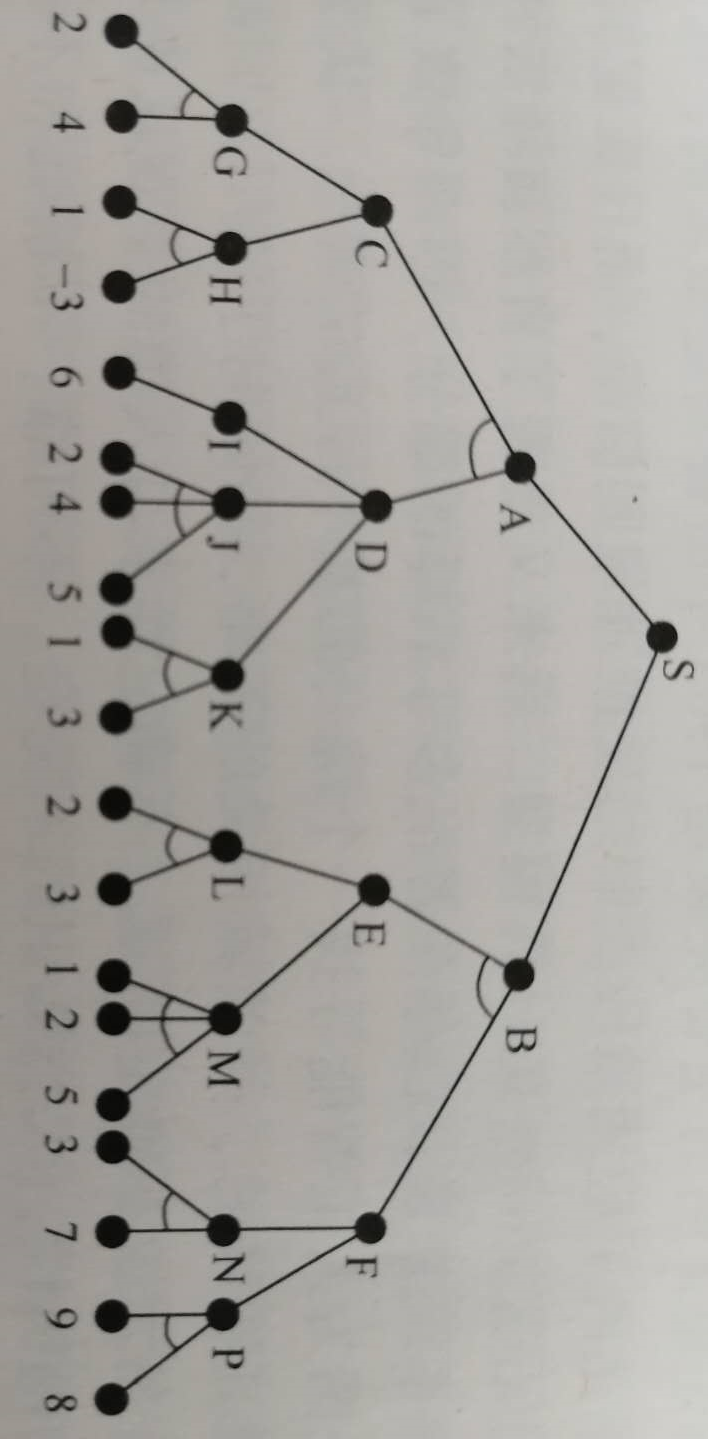
\includegraphics[angle=90,width=0.6\textwidth]{20200314174705.png}
    \caption{博弈树}
    \label{20200314174705fig51}
\end{figure}
\end{think}
%%%%%%------------------------------------
\begin{think}
    用matlab或Python语言实现图\ref{AI32fig51}博弈树的深度优先和宽度优先搜索算法, 并绘制流程图.
\end{think}
%%%%%%------------------------------------
\begin{custom}[explorecolor]{探索}
设有如下结构的移动将牌游戏:$$B\,\,	B\,\,		W\,\,		W\,\,		E,$$
其中, $B$表示黑色将牌, $W$表是白色将牌, $E$表示空格. 游戏的规定走法是:

(1) 任意一个将牌可移入相邻的空格, 规定其代价为1;

(2) 任何一个将牌可相隔1个其它的将牌跳入空格, 其代价为跳过将牌的数目加1.

游戏要达到的目标什是把所有$W$都移到$B$的左边. 对这个问题, 请定义一个启发函数$h(n)$, 并给出用这个启发函数产生的搜索树.
你能否判别这个启发函数是否满足下界要求? 在求出的搜索树中, 对所有节点是否满足单调限制?
\end{custom}




